\chapter{Dinámica de la Red de Caspasas}
\label{cap:Modelos}


La cascada apoptótica debe integrar información proveniente del entorno, a través de ligandos de la muerte o señales de supervivencia, con información del estado interno celular, como daño al ADN y estado de oxidación, para decidir si proceder con el programa de muerte celular. Para comprender la forma en que la red sopesa dicha información es necesario confeccionar un modelo que incluya los distintos módulos y poder contrastarlo con varios experimentos. En este capítulo presentaré el desarrollo de los modelos utilizados para describir el comportamiento del sistema bajo estudio. Comenzaré describiendo un modelo introducido en \cite{Corbat2018} que describe adecuadamente la dinámica de la red ante estímulos extrínsecos. Al detectar incongruencias entre las predicciones del modelo y los experimentos con estímulos intrínsecos, se encontró una retroalimentación faltante y se completó el modelo. Éste último fue presentado en \cite{Corbat2021} y se comprobó que además de describir la dinámica ante estímulos intrínsecos y extrínsecos, podía predecir resultados de experimentos previos de otros laboratorios.


%%%%%%%%%%%%%%%%%%%%%%%%%%%%%%%
\section{Adquisición del Cuerpo de Datos}


Siguiendo el protocolo descripto en el capítulo \ref{cap:MatMet}, se transfectaron células con los biosensores caracterizados en el capítulo \ref{cap:Biosensores} y se las estimuló con TNF-$\alpha$ o staurosporina, estímulos extrínseco e intrínseco respectivamente \citep{Sakamaki2009, Malsy2019}. Dado que en este caso contamos con tres biosensores de espectro distinto, la secuencia de adquisición de imágenes tuvo que ser modificada. Se incluyeron los canales rojo y azul, utilizándose 150~ms de exposición ya que la eficiencia de detección es menor en esos rangos. Es necesario considerar el tiempo necesario para cambiar de canal que es de 500~ms, demorándose 1.6~s en adquirir las imágenes correspondientes a los tres canales con sus respectivas dos polarizaciones (ver \cref{fig:tiempo_adq_tres_canales}). Nuevamente, se estimó que es posible adquirir imágenes correspondientes a 75 posiciones como mínimo antes de volver a la primer posición, manteniendo 5 minutos de resolución temporal. Esto correspondería a 1125 a 3000 células por experimento realizado.

\begin{figure}
    \centering
    \includegraphics[width=0.7\textwidth]{img/cap_4/tiempo_adq_tres_canales.pdf}
    \caption{\footnotesize{Esquema de los tiempos característicos de la adquisición secuencial de imágenes para cada canal y en cada polarización. En este caso se usaron 50~ms de tiempo de exposición para adquirir cada imagen del canal verde y 150~ms para cada una de los canales rojo y azul, 90~ms entre cada polarización y 500~ms para alternar entre canales. La platina motorizada necesita 2 segundos para cambiar de posición y entrar en foco. El tiempo necesario para cambiar la configuración de canal está incluido en el tiempo necesario para que la platina se traslade de una posición a otra.}}
    \label{fig:tiempo_adq_tres_canales}
\end{figure}

\begin{figure}[htb]
    \centering
    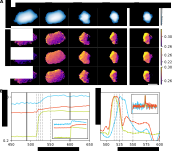
\includegraphics[width=0.8\textwidth]{img/cap_4/cels_anis.pdf}
    \caption{\footnotesize{Ejemplo ilustrativo del análisis de anisotropía. Adaptado de \cite{Habif2021}. \textbf{A.} Imágenes de fluorescencia y anisotropía de cada canal para una célula apoptótica. Se puede apreciar el aumento de anisotropía a distintos tiempos en cada canal. Cabe destacar que estas imágenes se generaron a modo ilustrativo y no fueron utilizadas para calcular las curvas de anisotropía. \textbf{B.} Curvas de anisotropía calculadas para la célula mostrada en \textbf{A}. El recuadro muestra la curva de anisotropía completa, las líneas verticales a trazos marcan los tiempos correspondientes a las imágenes, mientras que los rebordes oscuros corresponden a la sección de actividad graficada a la derecha.}}
    \label{fig:cels_anis}
\end{figure}

A partir del análisis de las imágenes, se obtuvieron las curvas de anisotropía para cada sensor en cada célula (ver \cref{fig:cels_anis} y \cref{fig:curvas_experimentales}). Luego, se generó un cuerpo de datos que contenía los tiempos de máxima actividad de las caspasas de las vías efectora, intrínseca y extrínseca de las 335 células apoptóticas, 152 estimuladas extrínsecamente y 183 de forma intrínseca. Como se mostró en la sección \ref{sec:Observable}, el tiempo de máxima actividad de cada caspasa sirve de referencia al tiempo de activación (ver \cref{fig:curvas_experimentales}). Es interesante notar que en ambos casos las caspasas extrínsecas y efectoras tienen un perfil sigmoideo, mientras que la intrínseca tiene un perfil hiperbólico.

\begin{figure}[htb]
    \centering
    \includegraphics[width=0.9\textwidth]{img/cap_4/all_experimental_curves.png}
    \caption{\footnotesize{Se transfectaron células HeLa con los biosensores de caspasas y se las expuso a estímulos extrínsecos e intrínsecos. \textbf{A.} Curva de anisotropía de ejemplo de una célula estimulada extrínsecamente. En este caso se utilizaron los sensores sCas3-BP, sCas8-RP y sCas9-GP. En el gráfico inferior se muestran las curvas de actividad obtenidas. Notar el perfil sigmoideo de las caspasas extrínsecas y efectoras, mientras que la intrínseca tiene un perfil hiperbólico. Adaptado de \cite{Corbat2018}. \textbf{B.} Curvas de anisotropía de ejemplo de una célula estimulada intrínsecamente. En este caso se utilizaron los sensores sCas8-BP, sCas9-RP y sCas3-GP. En el gráfico inferior se muestran las curvas de actividad obtenidas. Notar el perfil sigmoideo de las caspasas extrínsecas y efectoras, mientras que la intrínseca tiene un perfil hiperbólico. Adaptado de \cite{Corbat2021}.}}
    \label{fig:curvas_experimentales}
\end{figure}

Podemos apreciar una elevada variabilidad en el inicio de la cascada apoptótica, del orden de varias horas, utilizando el tiempo de máxima actividad de la caspasa efectora como referencia (ver \cref{fig:tiempos_experimentales}A). La diferencia entre los tiempos de activación de los distintos nodos es menos variable y del orden de minutos.  Luego, se calcularon las diferencias entre los tiempos de máxima actividad de las caspasas iniciadoras (caspasa 8 extrínseca y caspasa 9 intrínseca) y la efectora (caspasa 3). Se estimó un histograma de densidad utilizando funciones gaussianas para convolucionar con cada tiempo hallado (Kernel Density Estimation o KDE) y se graficaron las curvas de nivel que envolvían el 34\% y 68\% de los datos experimentales (ver \cref{fig:tiempos_experimentales}B). Podemos apreciar que prácticamente todos los tiempos, correspondientes a ambos estímulos caen en el primer cuadrante, lo que se traduce en que la caspasa efectora es la primera en alcanzar el máximo de actividad. En principio, uno esperaría que las caspasas iniciadoras sean las primeras en alcanzar el máximo de actividad, sin embargo, esto no ocurre debido a que éstas están fuertemente inhibidas y controladas. Una vez que la caspasa efectora alcanza el máximo de actividad, ésta retroalimenta a las iniciadoras, permitiéndoles alcanzar su máximo de actividad. Este mecanismo de inhibición de las iniciadoras y retroalimentación de la caspasa efectora evita que activaciones accidentales de caspasas iniciadoras desencadenen una respuesta completa. A su vez, si la caspasa efectora comenzará el proceso de apoptosis, la retroalimentación evitaría que pueda ser interrumpido culminando en una célula que sobrevive luego de haberse producido daño irreparable por parte de la caspasa efectora.

\begin{figure}[htb]
    \centering
    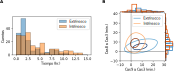
\includegraphics[width=0.9\textwidth]{img/cap_4/tiempos_experimentales.png}
    \caption{\footnotesize{Se estudiaron los tiempos de máxima actividad de cada caspasa y las relaciones entre ellos. De las 335 curvas apoptóticas, 152 correspondían a células estimuladas extrínsecamente y 183 a intrínsecamente estimuladas. Adaptado de \cite{Corbat2021}. \textbf{A.} Se confeccionaron histogramas del tiempo de máxima actividad de la caspasa efectora y se lo asoció con el inicio de la cascada apoptótica. Se pudo apreciar una elevada variabilidad, del orden de horas, en este desencadenamiento. \textbf{B.} Se analizaron las diferencias entre los tiempos de máxima actividad de las caspasas iniciadoras y la efectora. La caspasa efectora llega al máximo de actividad primera sin importar el estímulo utilizado. En el caso de células extrínsecamente estimuladas, la caspasa extrínseca 8 llegó al máximo de actividad $5_2^9$ minutos después que la caspasa efectora (mediana y rango intercuartil), mientras que la caspasa intrínseca 9 alcanza el máximo de actividad $8_5^{14}$ minutos después del máximo de actividad de la caspasa efectora. Al usarse estímulo intrínseco, la caspasa intrínseca fue la segunda en alcanzar el máximo de actividad $4_2^8$ minutos después de la efectora, mientras que la caspasa extrínseca lo alcanzó $9_5^{14}$ minutos después de la efectora.}}
    \label{fig:tiempos_experimentales}
\end{figure}

En el caso de células extrínsecamente estimuladas, la caspasa extrínseca 8 llegó al máximo de actividad $5_2^9$ minutos después que la caspasa efectora (mediana y rango intercuartil). Finalmente, la caspasa intrínseca 9 alcanza el máximo de actividad $8_5^{14}$ minutos después del máximo de actividad de la caspasa efectora. Por otro lado, al usarse estímulo intrínseco, la caspasa intrínseca fue la segunda en alcanzar el máximo de actividad $4_2^8$ minutos después de la efectora, mientras que la caspasa extrínseca lo alcanzó $9_5^{14}$ minutos después de la efectora. La distribución de puntos se ve afectada tanto por ruido en la determinación de los máximos de actividad, como por efecto de las demoras introducidas en los nodos por tener concentraciones distintas de biosensores y otras especies. Cabe destacar que el rango dinámico reducido de los sensores rojo y azul, hacen que la determinación de sus máximos sea más ruidosa (ver \cref{fig:tiempos_experimentales}).


%%%%%%%%%%%%%%%%%%%%%%%%%%%%%%%%%%%%
\section{Modelo de la Dinámica ante Estímulos Extrínsecos}


Se comenzó por estudiar y analizar distintos modelos en la bibliografía. \cite{Albeck2008} introdujeron en su trabajo un modelo que incluye los módulos extrínseco, intrínseco y efector con prácticamente todas las especies involucradas en la cascada (ver sección \ref{sec:intro:CascadaApoptotica} y \cref{fig:sketch_2018}). Considerando la completitud del modelo y el nivel de detalle que contiene, se decidió adaptarlo para incluir el comportamiento de los biosensores introducidos en el sistema. Para ello, se agregaron las especies correspondientes a cada biosensor en estado dimérico y se agregaron las reacciones por las cuales las caspasas se unen al biosensor y proceden a clivarlo.

\begin{figure}[htb]
    \centering
    \includegraphics[width=0.5\textwidth]{img/cap_4/model_simplified_noCas9FB.pdf}
    \caption{\footnotesize{Esquema simplificado del modelo de red de caspasas. Se pueden apreciar las ramas que intercomunican cada módulo. En particular, el módulo extrínseco activa el intrínseco y efector. El módulo intrínseco también activa el módulo efector. Y el módulo efector tiene una retroalimentación sobre el módulo extrínseco. Adaptado de \cite{Corbat2021}.}}
    \label{fig:sketch_2018}
\end{figure}

Es sabido que al incluir dichas especies en el modelo, también se deben seleccionar sus correspondientes parámetros. Para las constantes de reacción, se utilizaron las mismas constantes que cada caspasa tenía sobre sus sustratos. Teniendo en cuenta que el promotor viral utilizado genera una elevada concentración de biosensores, se utilizó una concentración inicial de 1.7~$\mu$M \citep{Wachsmuth2015}. Con el fin de incluir el efecto de de la variación en la concentración del biosensor, se tomaron valores de concentración inicial entre 5 y 10 $ \times 10 ^6$ moléculas por célula (siendo $10^7$ equivalente a 1.7~$\mu$M) y que resulta ser 5 a 10 veces la concentración de PARP, especie de concentración más alta del modelo. Se simuló el modelo 100 veces tomando valores distintos para la concentración inicial de cada biosensor y se estimó la señal de anisotropía a partir del estado del ensamble de cada biosensor. 

Las curvas de anisotropía generadas a partir de las simulaciones fueron analizadas de forma idéntica a las obtenidas experimentalmente. Éste modelo predice otro orden de activación de caspasas (ver \cref{fig:hist_extrinseco}) en el que las diferencias de tiempo caen en el segundo cuadrante, donde la caspasa intrínseca es la primera en alcanzar su máximo de actividad. Se analizaron qué parámetros del modelo podrían variarse para describir adecuadamente los tiempos obtenidos experimentalmente sin perder las predicciones de experimentos previos. Para empezar, sabiendo que el ligando de la muerte utilizado por \cite{Albeck2008} era distinto al que se utilizó en nuestros experimentos, comenzamos por variar las concentraciones iniciales de ligando y receptor. Usar una concentración de ligando y de receptor de $10^3$ moléculas por célula llevo a una descripción adecuada de la diferencia de tiempos entre la caspasa extrínseca y la efectora (ver \cref{fig:hist_extrinseco}A).

\begin{figure}[t!]
    \centering
    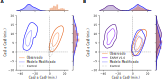
\includegraphics[width=0.9\textwidth]{img/cap_4/histogramas_extrinseco.png}
    \caption{\footnotesize{Gráficos de KDE con las predicciones de diferencia de tiempos entre máxima actividad de caspasas utilizando el modelo presentado por \cite{Albeck2008} modificado con la inclusión de los biosensores implementados y variando algunos parámetros. Se graficaron las curvas de nivel del KDE que encierran el 34\% y 68\% de los datos de diferencia de tiempos de máxima actividad observados experimentalmente (naranja) y el experimento control realizado con tres biosensores de caspasa 3 (gris). Adaptado de \cite{Corbat2018}. \textbf{A.} Se simuló cien veces el modelo variando la concentración inicial de los biosensores y fijando la concentración de ligando y receptor en $10^3$ (azul). \textbf{B.} Se simuló cien veces el modelo EARM 1.0 variando la concentración inicial de los biosensores (violeta) y luego se repitieron las simulaciones fijando la concentración inicial de ligando y receptor en $10^3$ y XIAP en $10^2$ (azul).}}
    \label{fig:hist_extrinseco}
\end{figure}

\begin{figure}[t!]
    \centering
    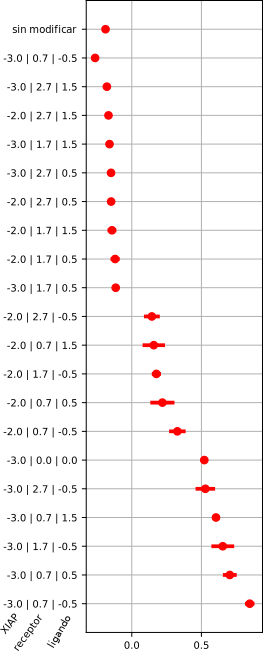
\includegraphics[width=0.4\textwidth]{img/cap_4/supplementary_4_A.pdf}
    \caption{\footnotesize{Se simuló el modelo EARM 1.0 modificado variando la concentración inicial del ligando, receptor y XIAP, multiplicándolos por 10 elevado al valor presentado. Se armaron histogramas bidimensionales con una cuadrícula de 4 a 6 minutos y se calculó la superposición con el histograma obtenido experimentalmente. Se vio que reducir la concentración de XIAP a $10^2$, el ligando a $10^3$ y aumentar la concentración del receptor a $10^3$ era la mejor combinación. Adaptado de \cite{Corbat2018}.}}
    \label{fig:cuad_min}
\end{figure}

A continuación, se buscó una especie que regule la diferencia entre tiempos de máxima actividad de la caspasa intrínseca y efectora sin afectar los otros resultados. Se vio que la proteína inhibidora de apoptosis ligada al cromosoma X (XIAP) inhibe a la caspasa efectora y a su vez es inhibida por Smac una vez liberada por la mitocondria post permeabilización de membrana. Reducir la concentración de XIAP a $10^2$ invierte el orden predicho entre la caspasa intrínseca y efectora, llegando a una descripción correcta de los tiempos entre caspasas (ver \cref{fig:hist_extrinseco}B). Para seleccionar los valores de las condiciones iniciales que mejor describan los resultados de tiempos experimentales, se construyeron los histogramas bidimensionales de diferencias de tiempo de máxima actividad para cada conjunto de parámetros y se calculó la superposición entre ambos (ver \cref{fig:cuad_min}).

Se verificó que el modelo modificado todavía predice los resultados presentados en el trabajo de \cite{Albeck2008}. Se corroboró que los anchos de las curvas de actividad sigan dentro de lo predicho previamente. Además se mantuvo el desencadenamiento abrupto posterior a la permeabilización de membrana, y se pudo apreciar el origen de la predicción realizada previamente donde la mayor parte de la caspasa extrínseca es activada debido a una retroalimentación. Este hecho acompaña nuestras observaciones experimentales donde la caspasa efectora alcanza el máximo de actividad antes que la extrínseca.


%%%%%%%%%%%%%%%%%%%%%%%%%%%%%%%%%
\section{Desarrollo de \textit{Apoptotic Reaction Model}}


Habiendo modificado el modelo para describir correctamente la diferencia entre tiempos de máxima actividad de caspasas al utilizar estímulos extrínsecos, se procedió a adaptarlo para predecir resultados en experimentos con estímulos intrínsecos. Dado que el modelo modificado contiene el módulo intrínseco, nos basamos en el trabajo de \cite{Zhang2009} para agregar una especie que simbolice el estímulo intrínseco. Dicha especie trunca a Bid, de la misma forma como lo hace la caspasa extrínseca. Se probaron distintos nodos para iniciar el estímulo, obteniendo resultados idénticos en todos los casos debido al desencadenamiento abrupto de la cascada post permeabilización de membrana mitocondrial.

Nuevamente, se simuló el sistema variando la concentración de los tres biosensores simultáneamente. A partir del estado del ensamble de biosensores se calcularon las correspondientes curvas de anisotropía, para luego analizarlas con el mismo protocolo que se usó en los experimentos. El modelo predecía que la caspasa intrínseca sería la primera en alcanzar la máxima actividad, seguida aproximadamente 30 minutos después por la efectora y otros 30 minutos después por la extrínseca (ver \cref{fig:exp_vs_Corbat}).

\begin{figure}[b!]
    \centering
    \includegraphics[width=0.9\textwidth]{img/cap_4/exp_vs_Corbat.png}
    \caption{\footnotesize{Gráficos de KDE con las predicciones de diferencia de tiempos entre máxima actividad de caspasas utilizando el modelo presentado en \cite{Corbat2018} modificado con la inclusión de estímulo intrínseco. Se simuló cien veces el modelo con cada estímulo variando la concentración inicial de los biosensores.  Adaptado de \cite{Corbat2021}. \textbf{A.} Se graficó la región que contiene a todas las curvas de anisotropía y actividad simuladas y se remarcó la curva cuya concentración corresponde a la mediana de concentraciones. En el modelado se usaron sCas3-BP, sCas8-RP y sCas9-GP. \textbf{B.} Se graficaron las curvas de nivel del KDE que encierran el 68\% de los datos de diferencia de tiempos de máxima actividad observados experimentalmente (celeste para extrínseco y naranja  para intrínseco) y el 34\% de las cien simulaciones (violeta para extrínseco y rojo  para intrínseco). Aunque la dinámica esta bien descripta por el modelo al usar estímulos extrínsecos, el orden de las caspasas efectora e intrínseca se encuentran invertidos al simularlo con estímulos intrínsecos.}}
    \label{fig:exp_vs_Corbat}
\end{figure}

En primer lugar, se barrieron las concentraciones iniciales de la caspasa 6, caspasa intrínseca, Apaf y citocromo C, así como las constantes cinéticas de activación de Apaf por el citocromo C, la conversión de Apaf en el apoptosoma, la inhibición de XIAP por Smac, la unión entre caspasa 6 y la caspasa extrínseca y las constantes de unión entre las caspasas y los tres biosensores. Todos estos parámetros fueron estudiados ya que controlan especies que se encuentran en la rama que conecta la caspasa intrínseca y la efectora. Aunque no se halló ninguna combinación de parámetros que genere un modelo capaz de describir experimentos con estímulo intrínseco y extrínseco al mismo tiempo, si fue posible trasladar las diferencias de tiempos para describir los experimentos con estímulo intrínseco, sacrificando los resultados previos (ver \cref{fig:CorbatForzado}). En este caso, el biosensor de caspasa intrínseca no llega a clivarse en su totalidad en el transcurso de las 15 horas simuladas.

\begin{figure}
    \centering
    \includegraphics[width=0.9\textwidth]{img/cap_4/force_corbat.png}
    \caption{\footnotesize{Gráficos de las predicciones utilizando el modelo presentado en \cite{Corbat2018} modificado con la inclusión de estímulo intrínseco y para que la diferencia de tiempos de máxima actividad de caspasas al utilizar estímulos intrínsecos esté bien descripta. Se simuló cien veces el modelo con cada estímulo variando la concentración inicial de los biosensores.  Adaptado de \cite{Corbat2021}. \textbf{A.} Se graficó la región que contiene a todas las curvas de anisotropía y actividad simuladas y se remarcó la curva cuya concentración corresponde a la mediana de concentraciones. En el modelado se usaron sCas3-BP, sCas8-RP y sCas9-GP. \textbf{B.} Se graficaron las curvas de nivel del KDE que encierran el 68\% de los datos de diferencia de tiempos de máxima actividad observados experimentalmente (celeste para extrínseco y naranja  para intrínseco) y el 34\% de las cien simulaciones (violeta para extrínseco y rojo  para intrínseco). Aunque la dinámica esta bien descripta por el modelo al usar estímulos intrínsecos, la diferencia de tiempos de máxima actividad de caspasas para estímulos extrínsecos esta muy alejada de lo esperado y en ambos casos el biosensor de caspasa intrínseca no llega a clivarse en su totalidad.}}
    \label{fig:CorbatForzado}
\end{figure}


%%%%%%%%%%%%%%%%%%%%%%%%%%%%
\subsection{Evaluación de Modelos Previos}


Dado que no se hallaron combinaciones de parámetros que sean capaces de describir experimentos con ambos estímulos, se consideró realizar un barrido de parámetros utilizando varios modelos previamente publicados. \cite{Lopez2013} desarrollaron un paquete de Python denominado PySB (por las siglas de \ening{Python Systems Biology}) que permite definir modelos numéricos de diversos tipos y simularlos. Por medio de este paquete, es posible definir módulos que se pueden integrar para formar un modelo completo.  Dentro de dicho paquete, hay una librería de modelos, entre los que se encuentran muchas variantes del modelo de Apoptosis. Se definió un pequeño módulo que agregaba los biosensores desarrollados al modelo en estudio. Se realizó un barrido grueso de los mismos parámetros en los modelos desarrollados por \cite{Howells2011, Albeck2008, Cui2008, Chen2007} y \cite{Chen2007a}. El modelo cuyas predicciones de tiempo de máxima actividad entre caspasas más se acercaba a los valores obtenidos experimentalmente fue el denominado Albeck11f, publicado por \cite{Albeck2008} (ver \cref{fig:albeck11f}). Aunque estas diferencias estaban descriptas adecuadamente, la forma funcional de los perfiles de actividad eran notoriamente distintos. En particular, el biosensor de la caspasa intrínseca no llegaba a clivarse por completo en las 15~hr simuladas.

\begin{figure}
    \centering
    \includegraphics[width=0.9\textwidth]{img/cap_4/albeck11f.png}
    \caption{\footnotesize{Gráficos de las predicciones utilizando el modelo presentado en \cite{Albeck2008}, llamado 11F, modificado con la inclusión de estímulo intrínseco y para que la diferencia de tiempos de máxima actividad de caspasas al utilizar ambos estímulos esté lo mejor descripta posible. Se simuló cien veces el modelo con cada estímulo variando la concentración inicial de los biosensores.  Adaptado de \cite{Corbat2021}. \textbf{A.} Se graficó la región que contiene a todas las curvas de anisotropía y actividad simuladas y se remarcó la curva cuya concentración corresponde a la mediana de concentraciones. En el modelado se usaron sCas3-BP, sCas8-RP y sCas9-GP. \textbf{B.} Se graficaron las curvas de nivel del KDE que encierran el 68\% de los datos de diferencia de tiempos de máxima actividad observados experimentalmente (celeste para extrínseco y naranja  para intrínseco) y el 34\% de las cien simulaciones (violeta para extrínseco y rojo  para intrínseco). Aunque las diferencias de tiempos están relativamente bien descriptas por el modelo al usar ambos estímulos, los perfiles de actividad se alejan de lo observado experimentalmente y en ambos casos el biosensor de caspasa intrínseca no llega a clivarse en su totalidad.}}
    \label{fig:albeck11f}
\end{figure}


%%%%%%%%%%%%%%%%%%%%%%%%%%%%%%%%%%%%
\subsection{Retroalimentación entre Caspasa Efectora e Intrínseca}
\label{sec:modelo:feedback}


Al analizar el orden de máxima actividad de las caspasas utilizando estímulos extrínsecos, notamos que la caspasa efectora era la primera en llegar al máximo de actividad y que ésta, a través de su retroalimentación mediante la caspasa 6, activaba lo remanente de la caspasa extrínseca, llegando así al máximo de actividad. De forma análoga, al utilizar estímulos intrínsecos, la caspasa efectora también alcanza su máximo de actividad en primer lugar y la sigue la caspasa intrínseca. A diferencia de la vía extrínseca, no se describe ninguna retroalimentación entre las caspasas efectora e intrínseca en el modelo. Sin embargo, al revisar la bibliografía, encontramos que diversos modelos preparados para describir experimentos con estímulos intrínsecos, incluyen una retroalimentación entre la caspasa efectora y la intrínseca \citep{Zhang2009, Rehm2006}. Adicionalmente, \cite{McComb2019} hacen especial hincapié en su trabajo en la importancia que tiene dicha retroalimentación. Desde el punto de vista molecular, el apoptosoma se encuentra preformado por Apaf-1, procaspasa 9 y dATP/ATP. El mismo es subsecuentemente activado al unírsele citocromo C, liberado post permeabilización de membrana mitocondrial y generando una variante denominada caspasa 9 (p35/p12), capaz de activar a la caspasa efectora. Ésta, a su vez, retroalimenta a la caspasa 9 y forma la subespecie p35/p10 que tiene mayor actividad enzimática y no es inhibida por XIAP.

Se reemplazó la conversión de un solo paso del apoptosoma por las reacciones descriptas previamente. Se utilizó la especie Apaf para representar al apoptosoma inactivo, y esta especie cambia a su estado activo luego de interactuar con el citocromo C citoplasmático. A continuación Apaf activo puede clivar a la caspasa 3 (representando a la efectora), así como al biosensor, con una constante de reacción baja. Finalmente, la caspasa 3 cliva a Apaf activo generando la especie Apop (que representa la caspasa 9 p35/p12), que tiene constantes catalíticas con sus sustratos mayores a Apaf activo y, además, no interactúa con XIAP (ver \cref{fig:sketch_2021}). Utilizando parámetros iguales a los anteriores, eligiendo la constante cinética de Apaf activo 10 veces menor que la de Apop, el modelo predice un orden de máxima actividad de caspasas acorde a lo observado experimentalmente.

\begin{figure}
    \centering
    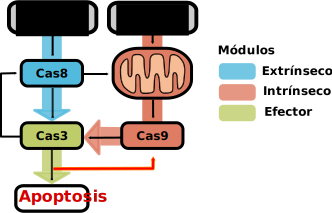
\includegraphics[width=0.5\textwidth]{img/cap_4/model_simplified.pdf}
    \caption{\footnotesize{Esquema simplificado del modelo de red de caspasas modelado. Se pueden apreciar las ramas que intercomunican cada módulo. En particular, el módulo extrínseco activa el intrínseco y efector. El módulo intrínseco también activa el módulo efector. Y el módulo efector tiene una retroalimentación sobre el módulo extrínseco e intrínseco. Adaptado de \cite{Corbat2021}.}}
    \label{fig:sketch_2021}
\end{figure}

Se utilizó el paquete de Python lmfit \citep{newville_2014} para hallar la mejor combinación de parámetros del modelo que describa los resultados obtenidos experimentalmente. Se utilizaron una búsqueda por cuadrilla (un método de fuerza bruta donde se varían las distintas combinaciones de todos los parámetros de forma equiespaciada) y luego \ening{Adaptive Memory Programming for Global Optimization} (AMPGO) \citep{Lasdon2010}. Los parámetros barridos fueron: las constantes de unión de todos los biosensores, Apaf activo al biosensor intrínseco y caspasa 3 a Apaf; así como las concentraciones iniciales de los biosensores, Apaf, XIAP y citocromo C. Los algoritmos utilizados buscaban minimizar las diferencias entre las predicciones de diferencias de tiempos de máxima actividad observadas y simuladas, y también, que el ancho de actividad de las caspasas sea el esperado. Los objetivos eran obtener 10 minutos de diferencia entre caspasa 9 y 3 y 5.5 minutos entre caspasa 8 y 3, al usar estímulo extrínseco; y 4 minutos entre caspasa 9 y 3 y 9 minutos entre caspasa 8 y 3 al utilizar estímulo intrínseco. Con todos los estímulos, se buscó un ancho de actividad de 15 minutos para la caspasa 3 y 8, y de 30 minutos para la caspasa 9. Una vez que ambos algoritmos hallaron la mejor combinación de parámetros, se hizo una mejora manual más fina de ellos. Éste modelo se llamó \textit{Apoptotic Reaction Model} (ARM, ya que surgió de \textit{Extrinsic Apoptotic Reaction Model} pero no es solo para estímulos extrínsecos) y se encuentra publicado en \cite{Corbat2021} y subido a \href{https://github.com/acorbat/caspase_model/tree/master}{caspase\textunderscore model} y \href{https://www.ebi.ac.uk/biomodels/MODEL2105210001}{Biomodels}  (ver apéndice \ref{repositorio}, \cite{Malik-Sheriff2018}).

Habiendo hallado la mejor combinación de parámetros, se simuló el modelo 100 veces variando la concentración inicial de los biosensores de forma correlacionada. Los tiempos obtenidos a partir del análisis de las curvas de anisotropía simuladas muestran un buen correlato con lo observado experimentalmente, así como los perfiles de actividad generados. En particular, se puede apreciar que la caspasa intrínseca tiene un perfil hiperbólico mientras que la efectora y extrínseca tienen un perfil sigmoideo (ver \cref{fig:ARM}). Cabe destacar que la concentración de las especies relacionadas a la caspasa intrínseca tienen un orden de magnitud menor que las propuestas previamente y, por lo tanto, se asemejan a estimaciones experimentales de su concentración.

\begin{figure}
    \centering
    \includegraphics[width=0.9\textwidth]{img/cap_4/arm.png}
    \caption{\footnotesize{Gráficos de las predicciones utilizando \textit{Apoptotic Reaction Model} \citep{Corbat2021}. Se simuló cien veces el modelo con cada estímulo variando la concentración inicial de los biosensores.  Adaptado de \cite{Corbat2021}. \textbf{A.} Se graficó la región que contiene a todas las curvas de anisotropía y actividad simuladas y se remarcó la curva cuya concentración corresponde a la mediana de concentraciones. En el modelado se usaron sCas3-BP, sCas8-RP y sCas9-GP. Al igual que en los experimentos (ver \cref{fig:curvas_experimentales}), la caspasa intrínseca tiene un perfil hiperbólico mientras que la efectora y extrínseca tienen un perfil sigmoideo. \textbf{B.} Se graficaron las curvas de nivel del KDE que encierran el 68\% de los datos de diferencia de tiempos de máxima actividad observados experimentalmente (celeste para extrínseco y naranja  para intrínseco) y el 34\% de las cien simulaciones (violeta para extrínseco y rojo  para intrínseco). La diferencia de tiempos de máxima actividad de caspasas para ambos estímulos se encuentra en concordancia con lo observado experimentalmente.}}
    \label{fig:ARM}
\end{figure}


%%%%%%%%%%%%%%%%%%%%%%%%%%%%%%%%
\section{Análisis de la Capacidad Predictiva}


A continuación, se evaluó la capacidad de ARM de describir resultados observados previamente sobre el comportamiento de la red apoptótica. En particular, se analizó el comportamiento de la red ante variaciones en la intensidad del estímulo utilizado \citep{Zhang2009, Albeck2008}, las susceptibilidades de la red ante variaciones en la concentración inicial de algunas especies \citep{Gaudet2012, Spencer2009, Rehm2006}, y la propagación de la señal ante ausencias de algunas caspasas específicas \citep{McComb2019, Inoue2009}.


%%%%%%%%%%%%%%%%%%%%%%%%%%%%
\subsection{Intensidad del estímulo}


El momento en que se desencadena la cascada apoptótica es, en promedio, inversamente proporcional a la intensidad del estímulo utilizado, tanto intrínseco como extrínseco \citep{Zhang2009, Albeck2008}. Para analizar este comportamiento, se simuló el modelo variando la intensidad de los estímulos a lo largo de 3 ordenes de magnitud. En ambos casos se pudo apreciar el comportamiento esperado (ver \cref{fig:BarridoEstimulo}A). Es interesante notar que las diferencias de tiempo de máxima actividad entre caspasas prácticamente no se ven afectadas por la intensidad del estímulo (ver \cref{fig:BarridoEstimulo}B). Aunque se puede ver que para estímulos extrínsecos hay un pequeño corrimiento, éste es del orden de unos pocos minutos y sería difícil de apreciar experimentalmente.

\begin{figure}
    \centering
    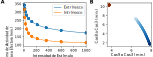
\includegraphics[width=0.7\textwidth]{img/cap_4/barrido_estimulo.pdf}
    \caption{\footnotesize{Se analizaron los efectos de variar la intensidad de los estímulos sobre los tiempos de máxima actividad de las caspasas en ARM.  Adaptado de \cite{Corbat2021}. \textbf{A.} Se graficaron los tiempos de máxima actividad de la caspasa efectora en función de la intensidad del estímulo utilizado. La dependencia entre el desencadenamiento de la apoptosis y la intensidad del estímulo es inversamente proporcional con ambos tipos de estímulos. \textbf{B.} Se graficaron la diferencia de tiempos de máxima actividad entre caspasas al utilizar ambos tipos de estímulos (naranja intrínseco y celeste extrínseco) a lo largo de tres ordenes de magnitud. Debido al desencadenamiento rápido de la cascada, la intensidad del estímulo intrínseco no varía la diferencia de tiempo de máxima actividad entre caspasas. Por otro lado, variar la intensidad del estímulo extrínseco introduce un pequeño cambio en las diferencias de tiempo de máxima actividad que sería difícil de distinguir experimentalmente.}}
    \label{fig:BarridoEstimulo}
\end{figure}

\begin{figure}[t!]
    \centering
    \includegraphics[width=0.5\textwidth]{img/cap_4/sweep_int_stim.png}
    \caption{\footnotesize{Gráficos que muestran la concentración en función del tiempo de especies mitocondriales ante estímulos intrínsecos de distintos ordenes de magnitud. En particular se graficaron los estados de multimerización de Bax activo, Mito activo que representa los poros en la membrana mitocondrial y la concentración de citocromo C citoplasmático, que es el resultado final de la permeabilización de la membrana mitocondrial. Es de notar que al formarse unos pocos poros en la membrana, la liberación de citocromo C ocurre rápidamente y de ahí el desencadenamiento rápido de la cascada apoptótica. Adaptado de \cite{Corbat2021}.}}
    \label{fig:desencadenamiento_rapido}
\end{figure}

Se corroboró además que se mantiene el comportamiento de desencadenamiento abrupto de la cascada una vez alcanzada la permeabilización de membrana mitocondrial. Esto se aprecia fácilmente al ver que utilizando distintos ordenes de intensidad de estímulo intrínseco, las especies contenidas dentro de la mitocondria se liberan rápidamente una vez que se forman unos pocos (1 a 3) poros en la membrana (ver \cref{fig:desencadenamiento_rapido}). Este comportamiento se vio experimentalmente y se describió en \cite{Albeck2008}.


%%%%%%%%%%%%%%%%%%%%%%%
\subsection{Sensibilidad de los Observables}


Se realizó un análisis de sensibilidad de los observables a las concentraciones iniciales (no nulas) de las distintas especies. Esto trae aparejado dos beneficios: por un lado brinda un mejor entendimiento de la red y cómo los distintos parámetros afectan a los observables; y además, permite simular el efecto sobre los observables de experimentos análogos a reducir o incrementar la concentración de alguna especie en particular. Para dicho análisis, se incrementó y disminuyó la concentración de cada condición inicial por separado en medio orden de magnitud y un orden de magnitud y se estimaron los siguientes observables: inicio de la cascada (tiempo del máximo de actividad de la caspasa efectora), diferencia entre tiempos de máxima actividad de las caspasas iniciadoras y la efectora, y el ancho del perfil de actividad de cada caspasa (definido como el ancho de la mitad del máximo de actividad). Para calcular la sensibilidad se utilizó

\begin{equation*}
S = \frac{dObs}{d log k} = \frac{Obs_{per} - Obs}{log 10^{f} k - log k} = \frac{Obs_{per} - Obs}{f}.
\end{equation*}

\noindent Dado que cada concentración inicial k se incrementó y redujo en un orden y medio orden de magnitud, el denominador solo tomará los valores de $\pm 1$ y $\pm -1/2$. Al no haber grandes diferencias entre variar uno o medio orden de magnitud, nos concentraremos en describir el caso donde se incrementó medio orden de magnitud cada concentración inicial.

\begin{figure}[t!]
    \centering
    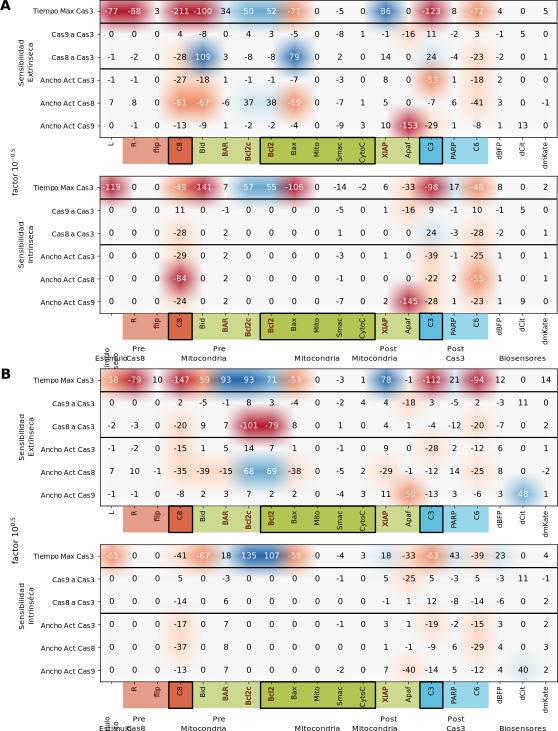
\includegraphics[width=0.7\textwidth]{img/cap_4/sensitivity_05.pdf}
    \caption{\footnotesize{Estudio de sensibilidad de los observables ante incrementar (\textbf{A}) y reducir (\textbf{B}) medio orden de magnitud cada concentración inicial del modelo. Los colores de cada elemento resaltan si hubo una diferencia apreciable en el observable. Las especies escritas en rojo con reborde negro corresponden a inhibidores. Adaptado de \cite{Corbat2021}.}}
    \label{fig:sensitividad05}
\end{figure}

\begin{figure}[t!]
    \centering
    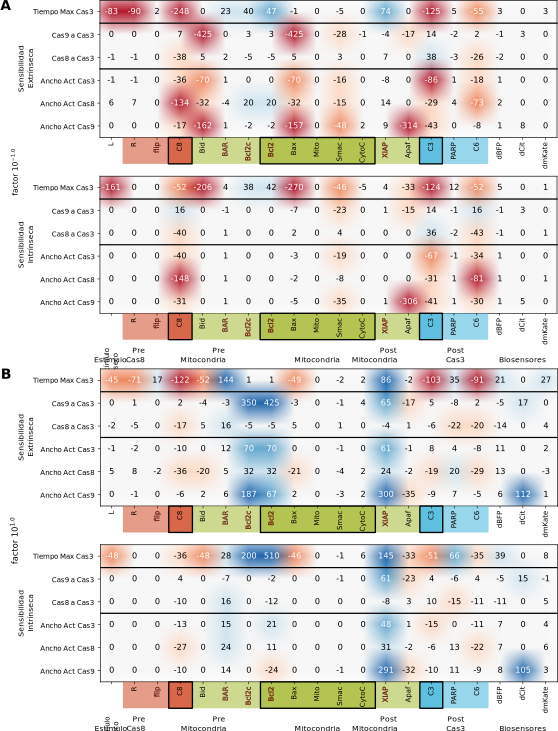
\includegraphics[width=0.7\textwidth]{img/cap_4/sensitivity_10.pdf}
    \caption{\footnotesize{Estudio de sensibilidad de los observables ante incrementar (\textbf{A.}) y reducir (\textbf{B.}) un orden de magnitud cada concentración inicial del modelo. Los colores de cada elemento resaltan si hubo una diferencia apreciable en el observable. Las especies escritas en rojo con reborde negro corresponden a inhibidores. Adaptado de \cite{Corbat2021}.}}
    \label{fig:sensitividad10}
\end{figure}

En el trabajo de \cite{Gaudet2012} se discuten en profundidad los efectos de variar las concentraciones iniciales de diversas especies sobre el momento en el que se desencadena la apoptosis al utilizar estímulos extrínsecos. Esto puede resumirse en como la sobreexpresión de inhibidores (FLIP, BAR, Bcl2 y XIAP) retrasan el inicio, mientras que caspasas, receptores y miembros proapotóticos de la familia BH3 la aceleran. Es de interés notar que Smac, citocromo C y Apaf no tienen ningún efecto. Estas predicciones están en acuerdo con experimentos realizados por \cite{Gaudet2012} para Bcl-2 y Bid y por \cite{Spencer2009} para FLIP y Bid. Análogamente, hay muchas similitudes con el análisis de sensibilidad al utilizar estímulos intrínsecos. Perturbaciones experimentales de Smac, XIAP y procaspasa 3 y 7 fueron realizadas por \cite{Rehm2006} y también acompañan lo descripto por el modelo. En particular, aumentar XIAP retrasa el inicio, las procaspasas 3 y 7 lo adelantan, mientras que Smac no tiene ningún efecto.

Al utilizar estímulos extrínsecos, la concentración inicial de Apaf y el biosensor de la caspasa intrínseca tienen un efecto sobre la diferencia de tiempos entre la caspasa efectora e intrínseca. El tiempo entre el máximo de actividad de la caspasa efectora y extrínseco se reduce levemente al aumentar Bcl-2 y la caspasa 6. En cuanto a las diferencias de tiempo de máxima actividad de caspasas al utilizar estímulos intrínsecos, Apaf afecta principalmente el tiempo entre caspasa efectora e intrínseca. De forma similar, el tiempo entre caspasa efectora y extrínseca se ve reducido por las especies involucradas en su retroalimentación como la caspasa 6 o la caspasa extrínseca. En contraposición, aumentar la concentración de la caspasa efectora, acelera su activación por retroalimentación y la adelanta respecto a la extrínseca, o también, aumentar los inhibidores de la caspasa extrínseca como BAR.

Estos resultados tienen valor tanto experimental ya que resumen qué concentraciones pueden afectar a cuáles observables, así como valor descriptivo del modelo ya que nos brindan información de qué parámetros no pueden ser precisamente determinados con los observables utilizados. Por otro lado, si uno necesitase modificar el modelo para incluir más experimentos, estas tablas dan cuenta de qué parámetros pueden modificarse sin afectar predicciones previas.


%%%%%%%%%%%%%%%%%%%%%%%%%%
\subsection{Propagación de la señal}

Por último, se simularon experimentos de 24~hr con ambos tipos de estímulos, llevando a cero la concentración de alguna o algunas caspasas para emular experimentos de \ening{Knock-Out} (KO). En los trabajos de \cite{Inoue2009} y \cite{McComb2019}, se knockean las caspasas 3, 6, 7, 8 y 9 o un subconjunto de ellas, para luego estimular las células de forma extrínseca o intrínseca. Luego de varias horas, se procede a lisarlas y estudiar la presencia de las distintas caspasas activas o inactivas mediante Western Blot. Aunque estos experimentos se realizaron en líneas celulares distintas a las que utilizamos previamente, esperamos que el comportamiento de la cascada sea similar. La propagación de la señal y las caspasas activas en cada situación descriptas por el modelo fueron las esperadas en acuerdo con lo observado experimentalmente (ver \cref{fig:KOCaspasas}).

\begin{figure}
    \centering
    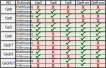
\includegraphics[width=0.7\textwidth]{img/cap_4/ko_table.pdf}
    \caption{\footnotesize{Se simularon experimentos en los que las concentraciones iniciales de un subconjunto de procaspasas se llevaba a cero para simular su KO. Se marcó con ticks cada caspasa que se halló activa en la simulación de 24~hr, mientras que se puso una cruz cuando su actividad fue nula o despreciable. En todos estos experimentos se obtuvo una predicción que se condice con el resultado experimental. Adaptado de \cite{Corbat2021}.}}
    \label{fig:KOCaspasas}
\end{figure}

Para empezar, dado que las caspasas 3 y 7 reconocen el mismo sitio de unión y son efectoras, los experimentos KO de alguna de ellas se simularon restando la mitad de la concentración inicial de caspasa efectora. Esto llevó a que simular KO de caspasa 3 ó 7 den resultados idénticos, donde se reduce la actividad de estas caspasas, pero se obtiene una respuesta completa de todas las caspasas en el largo plazo. Si se KO la caspasa 6 y se utiliza un estímulo extrínseco, se reduce levemente la dinámica de las caspasas, pero tampoco se aprecia una diferencia en el largo plazo. Contrariamente, si se utiliza un estímulo intrínseco, la caspasa extrínseca nunca llega a activarse. No nos debe sorprender que KO de la caspasa de la vía correspondiente al estímulo que se usa, resulta en que no haya actividad apreciable de ninguna caspasa (ver \cref{fig:KO_singles}).

\begin{figure}[b!]
    \centering
    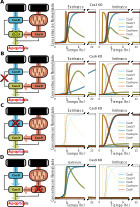
\includegraphics[width=0.75\textwidth]{img/cap_4/ko_singles.pdf}
    \caption{\footnotesize{Se simuló la cascada apoptótica llevando a cero la concentración de las procaspasas 3 (\textbf{A}), 6 (\textbf{B}), 8 (\textbf{C}) y 9 (\textbf{D}). Adaptado de \cite{Corbat2021}. \textbf{A.} Al hacer un KO de la caspasa 3, solo se ve una dinámica levemente más lenta que no será apreciable en experimentos de larga duración ya que ésta caspasa es redundante con la caspasa 7. \textbf{B.} Un KO de la caspasa 6 interrumpirá cualquier señal que pase de la caspasa efectora a la extrínseca. Es así que al usar estímulos extrínsecos, solo se ve una dinámica más lenta en la caspasa 8 por falta de retroalimentación, mientras que si se usan estímulos intrínsecos, la caspasa 8 nunca se activa. \textbf{C} y \textbf{D.} Al hacer KO de las caspasas iniciadoras, se bloquea todo actividad de caspasas al usar el estímulo correspondiente. Si se usa el estímulo opuesto al de la caspasa KO, entonces se observa actividad prácticamente normal.}}
    \label{fig:KO_singles}
\end{figure}

Doble KO de alguna caspasa efectora (3 ó 7) y la caspasa 6 llevó a células con una dinámica más lenta pero que culminaban en muerte celular. De forma similar a las células con KO de caspasa 6, al utilizar estímulos intrínsecos en estos casos, la caspasa extrínseca no llega a activarse. Aplicar un KO de ambas caspasas efectoras 3 y 7, con o sin caspasa 6 incluida, llevan a que no haya ninguna actividad de caspasa efectora. Utilizar estímulos extrínsecos llevan a que haya actividad de la caspasa extrínseca, pero la actividad de la caspasa intrínseca es despreciable. Además, si se utiliza un estímulo intrínseco en estos casos, no se puede apreciar actividad de ninguna caspasa, excepto la versión lenta de la caspasa intrínseca no completamente activa (descripta por \cite{Rehm2006} y en la sección \ref{sec:modelo:feedback}). En los experimentos esta actividad no se aprecia, probablemente debido a la degradación de especies que no fue incluida en el modelo. Cabe destacar que este comportamiento no puede ser descripto por los modelos previos ya que en todos ellos la retroalimentación a la caspasa intrínseca está ausente y ésta siempre se activaría por completo (ver \cref{fig:KO_dobles}).

\begin{figure}[b!]
    \centering
    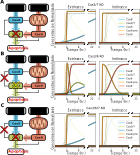
\includegraphics[width=0.75\textwidth]{img/cap_4/ko_multis.pdf}
    \caption{\footnotesize{Se simuló la cascada apoptótica llevando a cero la concentración de los subconjuntos de las procaspasas 3 y 7  (\textbf{A}); 3 y 6 (\textbf{B}); y 3, 6 y 7 (\textbf{C}). Adaptado de \cite{Corbat2021}. \textbf{A.} En las células KO para todas las caspasas efectoras, solo se aprecia actividad de la caspasa 9 (p35/p12) y de la caspasa 8 si el estímulo es extrínseco. \textbf{B.} Células sin caspasa 3 y 6, muestran una baja actividad de la caspasa efectora y una dinámica más lenta de la caspasa 8 (si son extrínsecamente estimuladas), pero normal en tiempos largos. \textbf{C} Si se KO las caspasas 3, 6 y 7, sólo se ve una actividad muy baja por parte de la caspasa 9 (p35/p12) que no podría ser apreciada experimentalmente y, si las células son estimuladas extrínsecamente, algo de actividad de la caspasa 8 también.}}
    \label{fig:KO_dobles}
\end{figure}

La adición de la retroalimentación entre las caspasas efectoras e intrínsecas sirvió tanto para recuperar la dinámica entre tiempos de máxima actividad entre caspasas como para incluir el comportamiento de la red ante experimentos de KO de caspasas. Cabe destacar que la variante p35/p12 de la caspasa intrínseca, al ser considerablemente más lenta que la variante p35/p10, permite reproducir resultados en los que las caspasas efectoras están knockeadas. Con los modelos previos, la única variante de la caspasa intrínseca se activa por completo una vez permeabilizada la membrana mitocondrial, mientras que en ARM solo se aprecia una baja actividad por parte de la variante p35/p12.